% Options for packages loaded elsewhere
\PassOptionsToPackage{unicode}{hyperref}
\PassOptionsToPackage{hyphens}{url}
\PassOptionsToPackage{dvipsnames,svgnames,x11names}{xcolor}
%
\documentclass[
]{article}

\usepackage{amsmath,amssymb}
\usepackage{iftex}
\ifPDFTeX
  \usepackage[T1]{fontenc}
  \usepackage[utf8]{inputenc}
  \usepackage{textcomp} % provide euro and other symbols
\else % if luatex or xetex
  \usepackage{unicode-math}
  \defaultfontfeatures{Scale=MatchLowercase}
  \defaultfontfeatures[\rmfamily]{Ligatures=TeX,Scale=1}
\fi
\usepackage{lmodern}
\ifPDFTeX\else  
    % xetex/luatex font selection
\fi
% Use upquote if available, for straight quotes in verbatim environments
\IfFileExists{upquote.sty}{\usepackage{upquote}}{}
\IfFileExists{microtype.sty}{% use microtype if available
  \usepackage[]{microtype}
  \UseMicrotypeSet[protrusion]{basicmath} % disable protrusion for tt fonts
}{}
\makeatletter
\@ifundefined{KOMAClassName}{% if non-KOMA class
  \IfFileExists{parskip.sty}{%
    \usepackage{parskip}
  }{% else
    \setlength{\parindent}{0pt}
    \setlength{\parskip}{6pt plus 2pt minus 1pt}}
}{% if KOMA class
  \KOMAoptions{parskip=half}}
\makeatother
\usepackage{xcolor}
\usepackage[lmargin=1.25in,rmargin=1.25in,tmargin=1in,bmargin=1in]{geometry}
\setlength{\emergencystretch}{3em} % prevent overfull lines
\setcounter{secnumdepth}{5}
% Make \paragraph and \subparagraph free-standing
\makeatletter
\ifx\paragraph\undefined\else
  \let\oldparagraph\paragraph
  \renewcommand{\paragraph}{
    \@ifstar
      \xxxParagraphStar
      \xxxParagraphNoStar
  }
  \newcommand{\xxxParagraphStar}[1]{\oldparagraph*{#1}\mbox{}}
  \newcommand{\xxxParagraphNoStar}[1]{\oldparagraph{#1}\mbox{}}
\fi
\ifx\subparagraph\undefined\else
  \let\oldsubparagraph\subparagraph
  \renewcommand{\subparagraph}{
    \@ifstar
      \xxxSubParagraphStar
      \xxxSubParagraphNoStar
  }
  \newcommand{\xxxSubParagraphStar}[1]{\oldsubparagraph*{#1}\mbox{}}
  \newcommand{\xxxSubParagraphNoStar}[1]{\oldsubparagraph{#1}\mbox{}}
\fi
\makeatother
\pagestyle{plain}


\providecommand{\tightlist}{%
  \setlength{\itemsep}{0pt}\setlength{\parskip}{0pt}}\usepackage{longtable,booktabs,array}
\usepackage{calc} % for calculating minipage widths
% Correct order of tables after \paragraph or \subparagraph
\usepackage{etoolbox}
\makeatletter
\patchcmd\longtable{\par}{\if@noskipsec\mbox{}\fi\par}{}{}
\makeatother
% Allow footnotes in longtable head/foot
\IfFileExists{footnotehyper.sty}{\usepackage{footnotehyper}}{\usepackage{footnote}}
\makesavenoteenv{longtable}
\usepackage{graphicx}
\makeatletter
\newsavebox\pandoc@box
\newcommand*\pandocbounded[1]{% scales image to fit in text height/width
  \sbox\pandoc@box{#1}%
  \Gscale@div\@tempa{\textheight}{\dimexpr\ht\pandoc@box+\dp\pandoc@box\relax}%
  \Gscale@div\@tempb{\linewidth}{\wd\pandoc@box}%
  \ifdim\@tempb\p@<\@tempa\p@\let\@tempa\@tempb\fi% select the smaller of both
  \ifdim\@tempa\p@<\p@\scalebox{\@tempa}{\usebox\pandoc@box}%
  \else\usebox{\pandoc@box}%
  \fi%
}
% Set default figure placement to htbp
\def\fps@figure{htbp}
\makeatother

\pagenumbering{gobble}
\usepackage{scrlayer-scrpage}
\rohead{PAMGuard Tethys in a Hurry V1.0}
\usepackage[noblocks]{authblk}
\renewcommand*{\Authsep}{, }
\renewcommand*{\Authand}{ and }
\renewcommand*{\Authands}{, }
\renewcommand\Affilfont{\small}
\makeatletter
\@ifpackageloaded{tcolorbox}{}{\usepackage[skins,breakable]{tcolorbox}}
\@ifpackageloaded{fontawesome5}{}{\usepackage{fontawesome5}}
\definecolor{quarto-callout-color}{HTML}{909090}
\definecolor{quarto-callout-note-color}{HTML}{0758E5}
\definecolor{quarto-callout-important-color}{HTML}{CC1914}
\definecolor{quarto-callout-warning-color}{HTML}{EB9113}
\definecolor{quarto-callout-tip-color}{HTML}{00A047}
\definecolor{quarto-callout-caution-color}{HTML}{FC5300}
\definecolor{quarto-callout-color-frame}{HTML}{acacac}
\definecolor{quarto-callout-note-color-frame}{HTML}{4582ec}
\definecolor{quarto-callout-important-color-frame}{HTML}{d9534f}
\definecolor{quarto-callout-warning-color-frame}{HTML}{f0ad4e}
\definecolor{quarto-callout-tip-color-frame}{HTML}{02b875}
\definecolor{quarto-callout-caution-color-frame}{HTML}{fd7e14}
\makeatother
\makeatletter
\@ifpackageloaded{caption}{}{\usepackage{caption}}
\AtBeginDocument{%
\ifdefined\contentsname
  \renewcommand*\contentsname{Table of contents}
\else
  \newcommand\contentsname{Table of contents}
\fi
\ifdefined\listfigurename
  \renewcommand*\listfigurename{List of Figures}
\else
  \newcommand\listfigurename{List of Figures}
\fi
\ifdefined\listtablename
  \renewcommand*\listtablename{List of Tables}
\else
  \newcommand\listtablename{List of Tables}
\fi
\ifdefined\figurename
  \renewcommand*\figurename{Figure}
\else
  \newcommand\figurename{Figure}
\fi
\ifdefined\tablename
  \renewcommand*\tablename{Table}
\else
  \newcommand\tablename{Table}
\fi
}
\@ifpackageloaded{float}{}{\usepackage{float}}
\floatstyle{ruled}
\@ifundefined{c@chapter}{\newfloat{codelisting}{h}{lop}}{\newfloat{codelisting}{h}{lop}[chapter]}
\floatname{codelisting}{Listing}
\newcommand*\listoflistings{\listof{codelisting}{List of Listings}}
\makeatother
\makeatletter
\makeatother
\makeatletter
\@ifpackageloaded{caption}{}{\usepackage{caption}}
\@ifpackageloaded{subcaption}{}{\usepackage{subcaption}}
\makeatother

\usepackage{bookmark}

\IfFileExists{xurl.sty}{\usepackage{xurl}}{} % add URL line breaks if available
\urlstyle{same} % disable monospaced font for URLs
\hypersetup{
  pdftitle={PAMGuard -- Tethys In A Hurry},
  pdfauthor={Douglas Gillespie; Marie Roch},
  colorlinks=true,
  linkcolor={blue},
  filecolor={Maroon},
  citecolor={Blue},
  urlcolor={Blue},
  pdfcreator={LaTeX via pandoc}}


\title{PAMGuard -- Tethys In A Hurry}


\author[1]{Douglas Gillespie}
\author[2]{Marie Roch}

\affil[1]{Sea Mammal Research Unit, University of St Andrews}
\affil[2]{Department of Computer Science, San Diego State University}


\date{2025-02-20}
\begin{document}
\maketitle

\centerline{\textbf{Tutorial Version 1.0}}
\vspace{3cm}

\centerline{\textbf{Learning Outcomes}}

This tutorial assumes you're familiar with both the PAMGuard Viewer and Tethys,
have both PAMGuard and Tethys installed and
running on your computer, and just need a quick guide to export some data:
\begin{enumerate}
\item Add a Tethys module to PAMGuard and connect to the Tethys Server
\item Understand relationships between PAMGuard data and Tethys documents
\item Export data from PAMGuard to Tethys:
\begin{itemize}
\item Calibration data
\item Deployment data
\item Detections
\end{itemize}
\item View the exported data both from within PAMGuard and using the Tethys Web client
\item Know where to go for help, or if things go wrong
\end{enumerate}
\newpage

\renewcommand*\contentsname{Table of contents}
{
\hypersetup{linkcolor=}
\setcounter{tocdepth}{3}
\tableofcontents
}
\listoffigures
\listoftables

\newpage{}

\pagenumbering{arabic}
\pagestyle{plain}

\section{Prerequisites}\label{prerequisites}

\subsection{Software Versions}\label{software-versions}

To run this tutorial you must have PAMGuard version 2.02.16 or later,
and Tethys sever Version 3.2 or later. The Tethys server must be running
on your computer. If you don't have these, or don't know how to set them
up, please complete the full PAMGuard Tethys tutorial available at
\href{https://www.pamguard.org/tutorials/tethys.html}{www.pamguard.org/tutorials/tethys.html}.

\subsection{Data}\label{data}

In principle, you can complete this tutorial with any data you like, so
long as those data have been processed with PAMGuard and you are able to
open and view the data with the
\href{https://www.pamguard.org/olhelp/overview/PamMasterHelp/docs/viewerMode.html}{PAMGuard
Viewer}. Again, if you don't know how to do this, we recommend that you
complete the earlier tutorial,
\href{https://www.pamguard.org/tutorials/staticmonitoring.html}{Introduction
to Static Monitoring}.

This tutorial picks up where the Static Monitoring tutorial left off,
using the pre-processed data available in the file
\href{https://zenodo.org/records/13880212}{viewer.zip available on
Zenodo}. If you've successfully completed that tutorial, you should use
the data that you've already processed yourself.

\subsubsection{Click Classification}\label{sec-species}

If you've downloaded the viewer data from the
\href{https://www.pamguard.org/tutorials/staticmonitoring.html}{Introduction
to Static Monitoring} tutorial, then you need to run the click
classifier on those data to separate out porpoise clicks. Refer to page
37 of that tutorial and complete the section ``Automatic
classification'' before proceeding here.

\section{Add the Tethys Module to
PAMGuard}\label{add-the-tethys-module-to-pamguard}

Open the data with the PAMGuard Viewer. If you don't already have it in
your PAMGuard configuration, from the \emph{File/Utilities} menu, add
the Tethys module.

Go to the Tethys tab in your PAMGuard display. If the top is orange
(Figure~\ref{fig-servererror}), then it's failed to connect to the
server, which means either that the server isn't running (so start it)
or PAMGuard is looking at the wrong server address. If you've launched
Tethys with it's default address (http://localhost:9779), then PAMGuard
will have worked. If you changed something in Tethys, then change
PAMGuard to match Tethys using the settings button just to the right of
the address. Once the server connection is established, PAMGuard will
revert to its default grey colour.

\begin{figure}

\centering{

\pandocbounded{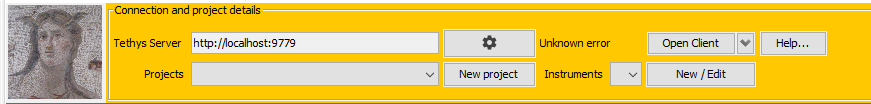
\includegraphics[keepaspectratio]{images/tethys1error.png}}

}

\caption{\label{fig-servererror}Tethys server errors colour the PAMGuard
display orange}

\end{figure}%

\section{Set Essential PAMGuard Metadata}\label{sec-metadata}

There are certain bits of information that are required by Tethys and
are also used to link to your PAMGuard dataset (a PAMGuard database and
binary store) to documents in Tethys.

\begin{enumerate}
\def\labelenumi{\arabic{enumi}.}
\tightlist
\item
  \textbf{Project} The Project name is a requirement of Tethys. The
  project label is text that helps you organize your data. It is usually
  used to provide a label for a group of instrument deployments that are
  related by geographic region, funding source, or purpose, and can
  serve as a useful filter when querying data. The dropdown box will
  show a list of all project names already available in the Tethys
  database you're using. You can select a name from the dropdown list,
  or press the `New Project' button to enter the name of a new one. A
  single Project may be associated with many PAMGuard datasets, for
  example, when deploying autonomous recorders, PAMGuard will have one
  dataset per recorder, or you may have multiple vessel based surveys
  which all form part of the same project, but will probably have one
  PAMGuard dataset per cruise.
\item
  \textbf{Instrument} The Instrument name is used to link specific
  Tethys Deployment documents back to a single PAMGuard dataset. The
  linkage uses both the Instrument name and the date range of the
  PAMGuard data, on the basis that it's impossible for the same
  instrument to be in two places at once. If it's not set, then press
  the \textbf{New/Edit} button (which will open the PAMGuard array
  dialog - Figure~\ref{fig-instrument}) and enter the information. The
  information consists of an instrument type, e.g.~something like
  MARU,or SoundTrap-HF600, and an Id, which should ideally be a
  manufacturer's serial number. If you don't have a serial number, then
  write something that can be used to identify the equipment,
  e.g.~Instrument Type: ``Home made array'', Instrument Id: ``2024 Mk
  2''.
\end{enumerate}

\begin{figure}

\centering{

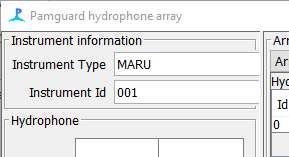
\includegraphics[width=0.45\linewidth,height=\textheight,keepaspectratio]{images/instrument.png}

}

\caption{\label{fig-instrument}Instrument identifying information in the
PAMGuard array dialog}

\end{figure}%

If you're working with the data from the Static Monitoring tutorial,
then use the following values for project and instrument
(Table~\ref{tbl-identify}). The latitude and longitude of the deployment
are also given here and will be used in the next step

\begin{longtable}[]{@{}ll@{}}
\caption{Essential project
information}\label{tbl-identify}\tabularnewline
\toprule\noalign{}
\endfirsthead
\endhead
\bottomrule\noalign{}
\endlastfoot
Project & Compass \\
Instrument Type & SoundTrap HF-300 \\
Instrument Id & 738725892 \\
Latitude & 56.09678 \\
Longitude & -8.02278 \\
\end{longtable}

\section{Export Calibration
information}\label{export-calibration-information}

\subsection{Set Values in PAMGuard}\label{set-values-in-pamguard}

Before exporting the calibration data, make sure that it's been
correctly set. Go back to the array manager dialog, either from the
\textbf{New/Edit} button next to the instrument id on the Tethys
display, or from the main PAMGuard menu \emph{Settings / Hydrophone
Array \ldots{}} (Figure~\ref{fig-badarray}).

\begin{figure}

\begin{minipage}{\linewidth}

\centering{

\pandocbounded{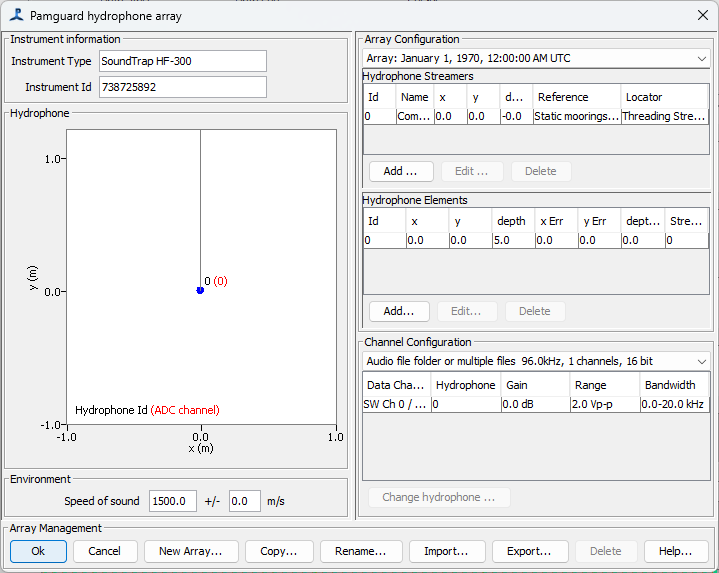
\includegraphics[keepaspectratio]{images/badarray.png}}

}

\subcaption{\label{fig-badarray}Array dialog information for the
SoundTrap tutorial dataset}

\end{minipage}%
\newline
\begin{minipage}{0.39\linewidth}

\centering{

\pandocbounded{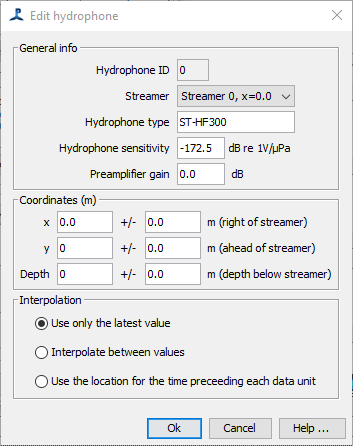
\includegraphics[keepaspectratio]{images/hydrophone.png}}

}

\subcaption{\label{fig-hydrophone}Correct hydrophone array settings}

\end{minipage}%
%
\begin{minipage}{0.01\linewidth}
~\end{minipage}%
%
\begin{minipage}{0.60\linewidth}

\centering{

\pandocbounded{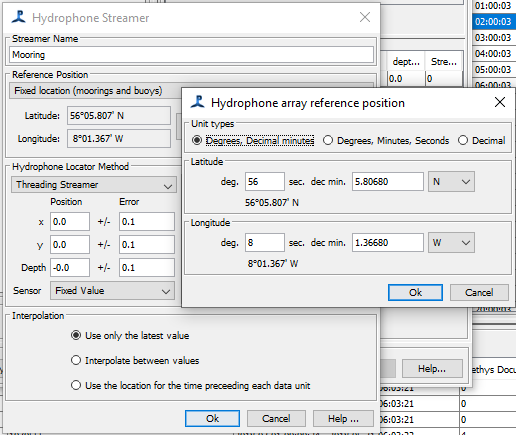
\includegraphics[keepaspectratio]{images/streamer.png}}

}

\subcaption{\label{fig-streamer}Corrected streamer information}

\end{minipage}%

\caption{\label{fig-arraymanager}PAMGuard Array management dialogs}

\end{figure}%

\begin{tcolorbox}[enhanced jigsaw, bottomtitle=1mm, toptitle=1mm, colback=white, toprule=.15mm, title=\textcolor{quarto-callout-important-color}{\faExclamation}\hspace{0.5em}{Important}, colbacktitle=quarto-callout-important-color!10!white, bottomrule=.15mm, breakable, opacitybacktitle=0.6, colframe=quarto-callout-important-color-frame, opacityback=0, left=2mm, titlerule=0mm, arc=.35mm, rightrule=.15mm, leftrule=.75mm, coltitle=black]

The calibration data may not have been set correctly in data from the
earlier tutorial, so you need to check it. When you look at the array
data, if it's showing two hydrophones, delete the second of them. Then
check the calibration and array location data.

\end{tcolorbox}

Next, edit the hydrophone data by double clicking on the hydrophone
element. (Figure~\ref{fig-hydrophone}): Enter the type as ST-HF300, the
sensitivity as -172.5, and the x,y,z coordinates all as zero.

Close that dialog with the OK button, then go to the `Streamer', but
selecting the one at the top that has a reference of a ``Ship GPS Data''
and press \textbf{Edit}.

Enter a name (though this won't be exported to Tethys), and select the
Reference Position as ``Fixed Location (moorings and buoys)''. Then
click on the little menu symbol next to the empty Latitude and Longitude
fields and set the correct values for the array location. You'll find it
easy to copy and paste the correct values (Table~\ref{tbl-identify}) if
you select Decimal display at the top of the dialog
(Figure~\ref{fig-streamer}).

\begin{tcolorbox}[enhanced jigsaw, bottomtitle=1mm, toptitle=1mm, colback=white, toprule=.15mm, title=\textcolor{quarto-callout-important-color}{\faExclamation}\hspace{0.5em}{Complete Calibration Data}, colbacktitle=quarto-callout-important-color!10!white, bottomrule=.15mm, breakable, opacitybacktitle=0.6, colframe=quarto-callout-important-color-frame, opacityback=0, left=2mm, titlerule=0mm, arc=.35mm, rightrule=.15mm, leftrule=.75mm, coltitle=black]

Calibration information is not just about the hydrophone. When dealing
with digital data, we also need to know how the amplitude of the numbers
in the sound files relate to the voltages in the wire generated by the
hydrophone.

The hydrophone calibration values we've entered above are only telling
us half the story, so it's essential that you also tell PAMGuard how
sensitive your recording system was. In PAMGuard this is set as a
``Peak-Peak voltage range'' in the sound acquisition dialog. For
SoundTraps, this should be set to 2. See the SoundTrap manuals from
\href{https://www.oceaninstruments.co.nz/}{Ocean Instruments} for
further information.

\end{tcolorbox}

\subsection{Run the Export Wizard}\label{run-the-export-wizard}

\begin{figure}

\begin{minipage}{0.49\linewidth}

\centering{

\pandocbounded{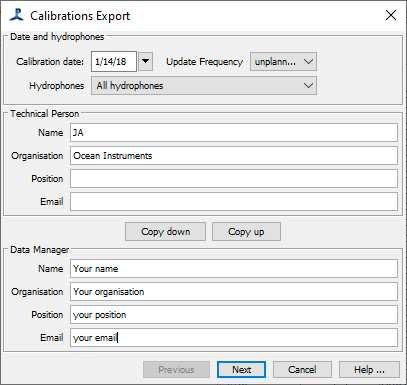
\includegraphics[keepaspectratio]{images/cal1.png}}

}

\subcaption{\label{fig-cal1}Calibration information panel}

\end{minipage}%
%
\begin{minipage}{0.02\linewidth}
~\end{minipage}%
%
\begin{minipage}{0.49\linewidth}

\centering{

\pandocbounded{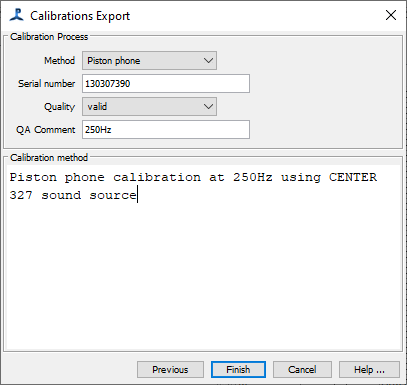
\includegraphics[keepaspectratio]{images/cal2.png}}

}

\subcaption{\label{fig-cal2}Calibration details panel}

\end{minipage}%

\caption{\label{fig-calwiz}Calibration Export Wizard pages}

\end{figure}%

Once all data in PAMGuard are correct, you can run the export wizard
which will create a Tethys document and write it to the database. To
start the process, press the \textbf{Export} button in the ``Instrument
Calibration Information'' section of the display - that's just under the
image of the Tethys Roman mosaic.

You'll then be asked for more information about the calibration process
(Figure~\ref{fig-calwiz}). The calibration was performed using a piston
phone calibrator at 250Hz, though we don't know the details of the
methodology. Fill in what you can. Table~\ref{tbl-caldata} is the
information we extracted from the calibration certificate for this
instrument.

\begin{longtable}[]{@{}ll@{}}
\caption{Data from the SoundTrap calibration
certificate}\label{tbl-caldata}\tabularnewline
\toprule\noalign{}
\endfirsthead
\endhead
\bottomrule\noalign{}
\endlastfoot
Date & 14 Jan 2018 \\
Operator & JA \\
Source Model & CENTER 327 \\
Source Serial & 130307390 \\
Frequency & 250Hz \\
Coupler & OIC1 \\
\end{longtable}

\section{Export Deployment data}\label{sec-deployments}

A key aspect of Tethys is recording why we collected data, as well as
how. This is essential in many studies that might use these data. For
example, if recorders were placed in a pseudo random pattern across a
study area, they they are much more suitable for abundance estimation
than recorders that were placed in a known hotspot for a particular
species. Being verbose with this information as you export the
deployment data is therefore essential if the data are going to be
useful in years to come.

These data were collected on a duty cycle of 20 minutes recording each
hour. There are therefore over 2000 entries in the recordings period
table. Right click on the table and \emph{Select All} from the popup
menu to export the whole lot as a single, duty cycled, deployment
document For more complex situations, such as ad-hoc deployments from
vessels, see the online help.

Press the \textbf{Export} button to start the Deployment Export dialog.
Again, you'll be asked for several pages of information about what you
were doing and why (Figure~\ref{fig-deploywiz}). The information you
need can mostly be copied from the project website at
\href{https://www.sams.ac.uk/science/projects/compass/}{www.sams.ac.uk/science/projects/compass/}.

\begin{figure}

\begin{minipage}{0.49\linewidth}

\centering{

\pandocbounded{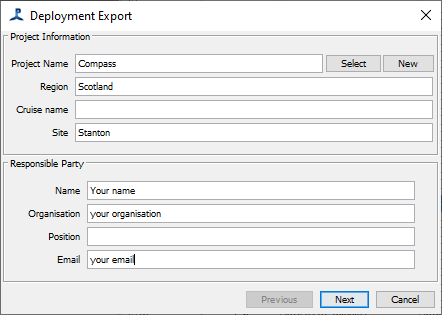
\includegraphics[keepaspectratio]{images/depl1.png}}

}

\subcaption{\label{fig-depl1}Project Information}

\end{minipage}%
%
\begin{minipage}{0.01\linewidth}
~\end{minipage}%
%
\begin{minipage}{0.49\linewidth}

\centering{

\pandocbounded{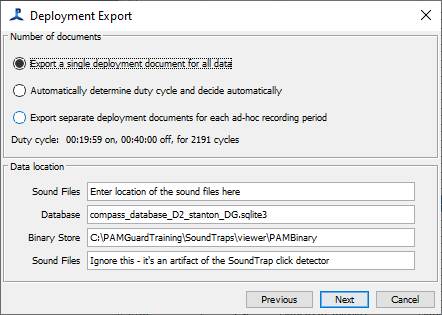
\includegraphics[keepaspectratio]{images/depl2.png}}

}

\subcaption{\label{fig-depl2}Deployment Effort}

\end{minipage}%
\newline
\begin{minipage}{\linewidth}

\centering{

\pandocbounded{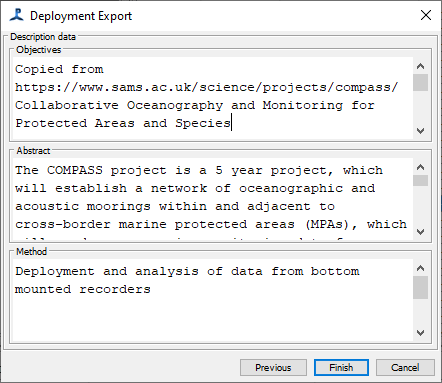
\includegraphics[keepaspectratio]{images/depl3.png}}

}

\subcaption{\label{fig-depl3}Deployment Description}

\end{minipage}%

\caption{\label{fig-deploywiz}Deployment Export Wizard pages}

\end{figure}%

\section{Export Detections}\label{export-detections}

Output from each detector in PAMGuard must be exported separately.
Available outputs are listed in the lower left panel of the display.

\subsection{Species Codes}\label{species-codes}

Before you can export data, you must set \href{https://itis.gov/}{ITIS
species codes} for the detector data that you're planning to export. To
do this, right click on the appropriate row in the table (in this case,
we'll pick the SoundTrap Click Detector Clicks) and select \emph{Species
Info \ldots{}} from the popup menu. Two species should be defined, one
for clicks that haven't been classified, and one for porpoise clicks
(Figure~\ref{fig-species1}). If this isn't the case, then you've
probably not set up and run the species classifier
(Section~\ref{sec-species}). For each, press the `Find' button and enter
an appropriate search term (Figure~\ref{fig-species2}) (e.g.~porpoise,
cetacean, odontoceti). PAMGuard will search the database for possible
matches and display a list of options. Select the species / taxa you
want. Then also fill in the Call / Sound type information, which is
important for species which have more than one call type (e.g.~clicks/
whistles). For further information see the
\href{https://www.pamguard.org/olhelp/utilities/tethys/docs/tethys_speciescodes.html}{PAMGuard
online help};

\begin{figure}

\begin{minipage}{0.49\linewidth}

\centering{

\pandocbounded{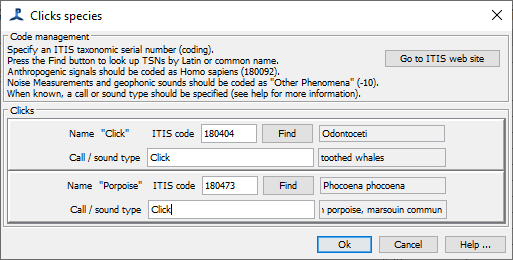
\includegraphics[keepaspectratio]{images/species1.png}}

}

\subcaption{\label{fig-species1}Dialog showing all species for a
detector}

\end{minipage}%
%
\begin{minipage}{0.01\linewidth}
~\end{minipage}%
%
\begin{minipage}{0.49\linewidth}

\centering{

\pandocbounded{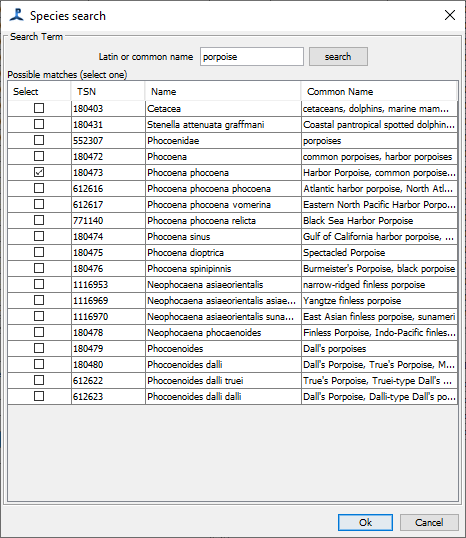
\includegraphics[keepaspectratio]{images/species2.png}}

}

\subcaption{\label{fig-species2}Searching for a specific species}

\end{minipage}%

\caption{\label{fig-species}PAMGuard dialogs for setting species codes}

\end{figure}%

\subsection{Granularity}\label{granularity}

Think about the granularity you want to export data at. This dataset
contains over a million clicks, and you probably don't want to export
all of them. Might you be better off exporting binned data (counts of
detections in a set time interval), or encounter data (counts of
detections without a gap between them) ? For this example, we'll export
encounter level data with an encounter defined as at least 10 clicks and
a 10 minute gap from adjacent encounters.

\subsection{Run The Export Wizard}\label{run-the-export-wizard-1}

\begin{figure}

\begin{minipage}{0.33\linewidth}

\centering{

\pandocbounded{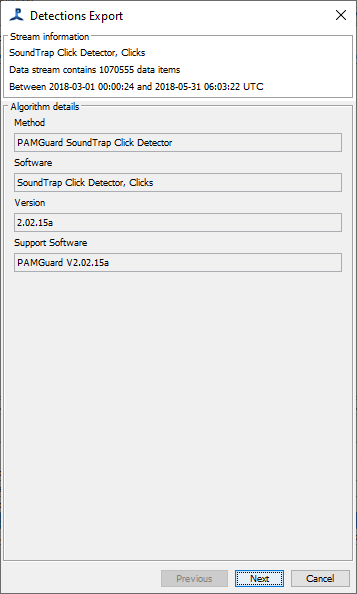
\includegraphics[keepaspectratio]{images/export1.png}}

}

\subcaption{\label{fig-export1}Detector information}

\end{minipage}%
%
\begin{minipage}{0.33\linewidth}

\centering{

\pandocbounded{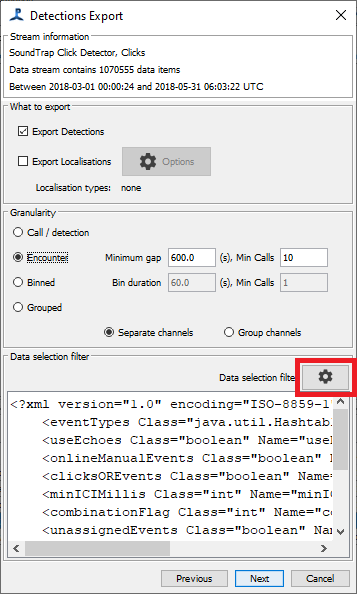
\includegraphics[keepaspectratio]{images/export2a.png}}

}

\subcaption{\label{fig-export2}Granularity and filtering}

\end{minipage}%
%
\begin{minipage}{0.33\linewidth}

\centering{

\pandocbounded{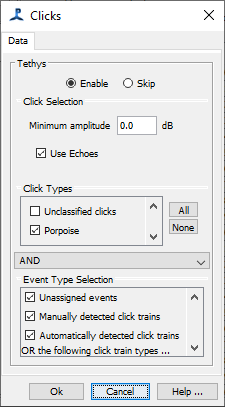
\includegraphics[keepaspectratio]{images/export3.png}}

}

\subcaption{\label{fig-export3}Data Selection Filter}

\end{minipage}%
\newline
\begin{minipage}{0.33\linewidth}

\centering{

\pandocbounded{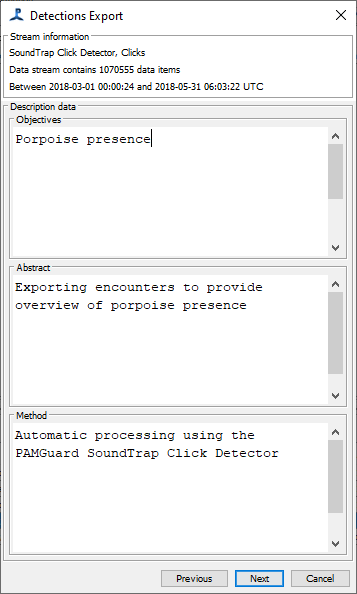
\includegraphics[keepaspectratio]{images/export4.png}}

}

\subcaption{\label{fig-export4}Additional Information}

\end{minipage}%
%
\begin{minipage}{0.33\linewidth}

\centering{

\pandocbounded{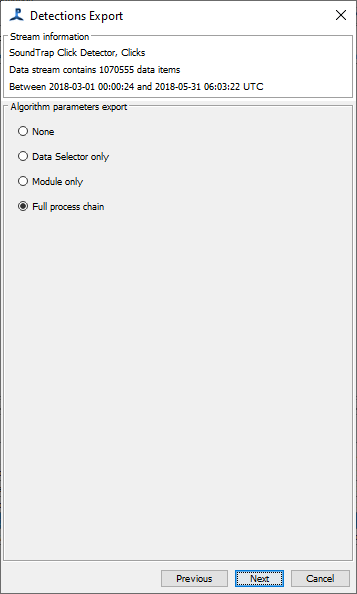
\includegraphics[keepaspectratio]{images/export5.png}}

}

\subcaption{\label{fig-export5}Detector Settings Output}

\end{minipage}%
%
\begin{minipage}{0.33\linewidth}

\centering{

\pandocbounded{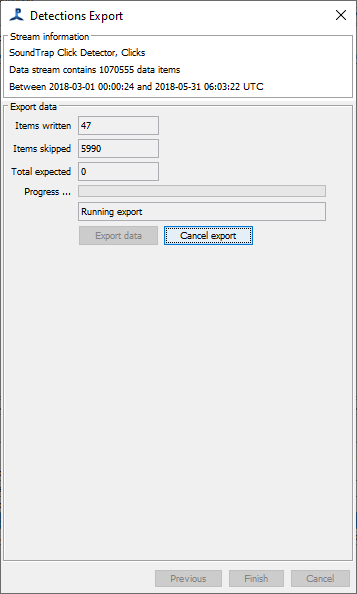
\includegraphics[keepaspectratio]{images/export6.png}}

}

\subcaption{\label{fig-export6}Export progress}

\end{minipage}%

\caption{\label{fig-export}Detections Export Wizard pages}

\end{figure}%

One the species codes are set, you can press the \textbf{Export} button
to start the export wizard (Figure~\ref{fig-export}). The first page
pulls information about the detector automatically from PAMGuard. On the
second page, you select whether you're exporting Detections or
Localizations, the Granularity, and importantly set an optional data
filter. The data filter is essential for many PAMGuard detectors, such
as the Click Detector, which generally run at quite a high false alarm
rate, before using an additional classifier to label the clicks of
interest. Press the button next to the Data Selection Filter (red box in
Figure~\ref{fig-export2}) and configure it to only select porpoise
clicks\footnote{Output from different detectors in PAMGuard often have
  different properties, so the Data Selection Filter you see will be
  different for each detector. See the PAMGuard online help for
  information about data selectors for specific detectors.}
(Figure~\ref{fig-export3}).The settings of the data filter will be
included in the detector parameters written to Tethys to provide a full
record of choices made during the export process.

On the next page (Figure~\ref{fig-export4}) add further information that
will help inform anyone using these data. These fields are similar to
those you filled in when exporting the Deployment information
(Section~\ref{sec-deployments}) but require different information. For
example, the Deployment information might contain quite general
information along the lines of ``Sound Trap deployments to detect small
cetaceans'', but the analysis so far has only dealt with Harbour
Porpoise. Perhaps you configured the detector to only detect buzzes, and
not regular clicks, etc. you need to include information about what you
actually did with the data, which is different to what MIGHT be done
with the data here.

Once you get to the last page, press the \textbf{Export Data} button and
wait while PAMGuard chugs through, loading a file at a time, extracting
the clicks that pass the selection filter, creating Encounters, or
Binned Data, and then finally writing the document.

Once the export process is complete, a dialog will show to indicate
success and a record will show in the table in the bottom right corner
of the display (Figure~\ref{fig-success}). Note that for this export, by
selecting to only export porpoise clicks, and exporting them as
encounters, only 616 Detection records were created from a total of
1070555 click in the data.

\begin{figure}

\centering{

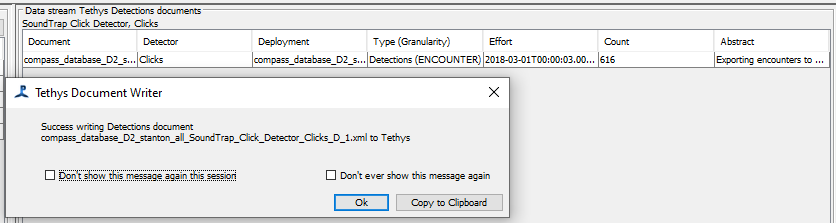
\includegraphics[width=0.9\linewidth,height=\textheight,keepaspectratio]{images/success.png}

}

\caption{\label{fig-success}Message shown on completion of a successful
export}

\end{figure}%

\section{View your data in PAMGuard}\label{view-your-data-in-pamguard}

The Tethys Client and Data Explorer offer by far the best and most
flexible interface for viewing Tethys data. However, PAMGuard does allow
a quick view of exported documents which can be useful to verify that
data have exported correctly.

\subsection{Web Client}\label{web-client}

Assuming that the server is running, and PAMGuard is successfully
connected to the server, then simply press the \textbf{Open Client}
button at the top of the display. This will open the Tethys Web Client
in your default web browser. To view listings of Documents of a
particular type (Calibrations, Deployments, etc.), to to the small menu
in the very top right of the web page, to the right of the Tethys mosaic
image.

\subsection{PAMGuard Quick View}\label{pamguard-quick-view}

Each section of the display will show which documents have been
exported. For the Detections, this is the separate table in the bottom
right of the display, since each module in PAMGuard might be exported to
multiple documents. When you select a PAMGuard datablock in the bottom
left table, the bottom right table will populate with documents
associated with that detector.

You can right click on the appropriate table row and select to view the
document, which will open in a new window (Figure~\ref{fig-docview}).

\begin{figure}

\centering{

\pandocbounded{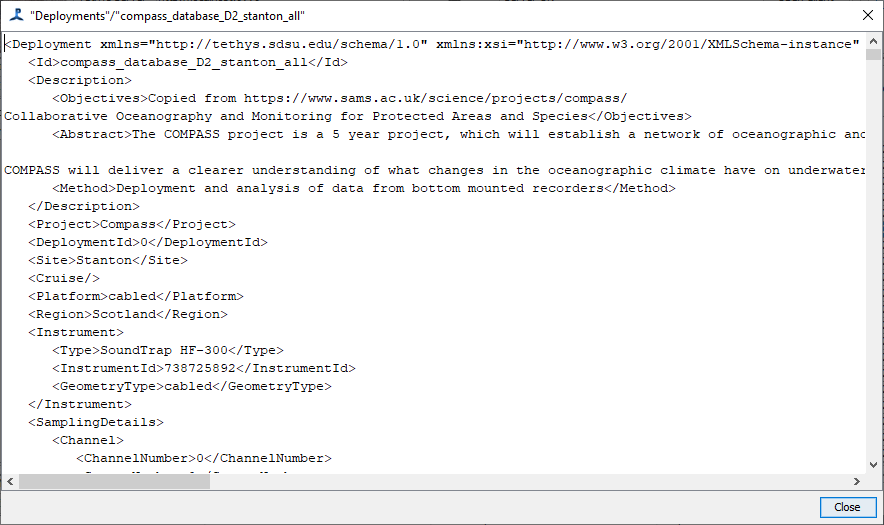
\includegraphics[keepaspectratio]{images/docview.png}}

}

\caption{\label{fig-docview}Example of a Deployment document viewed
within PAMGuard}

\end{figure}%

You can also use the small down pointing arrow to the right of the
\textbf{Open Client} button in the connection panel at the top of the
display to open lists of all documents in the database, either using the
Tethys Client, or in PAMGuard.

Open the Deployment document you created earlier and you will see the
information you entered during the export process
(Figure~\ref{fig-docview}).

\subsection{Delete Exported Documents}\label{delete-exported-documents}

As with viewing documents, the same right click actions and the PAMGuard
documents list can be used to delete documents.

\section{Problems}\label{problems}

\subsection{Problems exporting}\label{problems-exporting}

If PAMGuard fails to export a document to Tethys, an error message will
appear on the screen. Please copy the text from this message (there is a
copy button in the corner of the pop-up window) and send it to us at
\href{mailto:support@pamguard.org}{\nolinkurl{support@pamguard.org}}.

Just prior to export, PAMGuard saves a text copy of each document in a
temporary folder. This will be something like
C:\textbackslash Users\textbackslash{}\emph{yourusername}\textbackslash AppData\textbackslash Local\textbackslash Temp\textbackslash PAMGuardTethys.
You can find this folder most easily simply by going back to the little
menu to the right of the \textbf{Open Client} button and selecting
\emph{Open temp folder} from the bottom of the menu. Here you should
find a copy of the document that failed to export, (though it may get
deleted when you exit PAMGuard). If you can attach that to your email,
it will help us to quickly assess what went wrong and try to fix the
problem in future releases.

\subsection{PAMGuard viewer not finding Tethys
data}\label{pamguard-viewer-not-finding-tethys-data}

When you close and re-open the PAMGuard viewer that you exported data
from, then if the Tethys server is running PAMGuard should automatically
display the documents associated with that dataset. If this doesn't
happen, then first open the Client, and check that you can see the
documents there. If the documents exist, then the most likely cause is
that you've changed the Project name, the Instrument name, or the
Instrument Id in the Array Manager all of which are used to associate a
PAMGuard dataset with a set of Tethys documents
(Section~\ref{sec-metadata}).

\section{Further Learning}\label{further-learning}

\subsection{Tethys}\label{tethys}

There is extensive documentation for the Tethys Client and the Data
Explorer which you should find in both MS Word and PDF format in the
Documentation folder of your Tethys Installation. There, you'll also
find out about how to import data into R and Matlab. One of the
documents is called ``READ ME FIRST.docx'', so start there.

\subsection{PAMGuard Batch Processing}\label{pamguard-batch-processing}

This `in a Hurry' tutorial has run to over 10 pages, and I'm sure you
don't want to go through all of the steps above for every set of data
you've collected. The good news is that you probably don't have to. The
latest version (2.0 or later) of the batch processor module can run
export tasks on multiple PAMGuard datasets fully (or at least mostly)
automatically. To learn more about this, complete the latest Batch
Processing and Batch Output to Tethys tutorials available at
(\textbf{link to follow}).




\end{document}
